% In the current task there is only one label, so the label distribution is not a challenge. Therefore, a low misclassification rate or respectively a high accuracy rate can be treated as an algorithm result of very high quality \cite{luckert2016using}. 

% On one side, to improve the segmentation algorithm's accuracy, both false positives and false negatives were identified, labelled and added to the data set. 

% On the other side, to improve the pose algorithm's accuracy, different approaches were taken. For example, in the MAV algorithm an offset was calculated and added manually, and an averaging mechanism was added to calculate the cow teat's tip. 

% Subsequently, a correlogram was used to analyze the influence of the camera position and orientation on the error estimation. The correlation coefficients proved a strong indirect correlation and the error showed to be normally distributed. 

% Therefore, linear models are a promising step for predicting and subtracting the error. 
% % It is part of the further steps in Chapter \ref{chap:conclusion} to minimize the error offset using a separate algorithm. 
% To compare the algorithms among each other, the average error from the errors in (x,y,z) against the cow teat's tip ground truth was evaluated. 







% \section{Implementation}\label{chap:3:implementation-architecture}
% \section{Experiments}\label{chap:3:experiments}

% \begin{figure}[!ht]
%         \centering
%         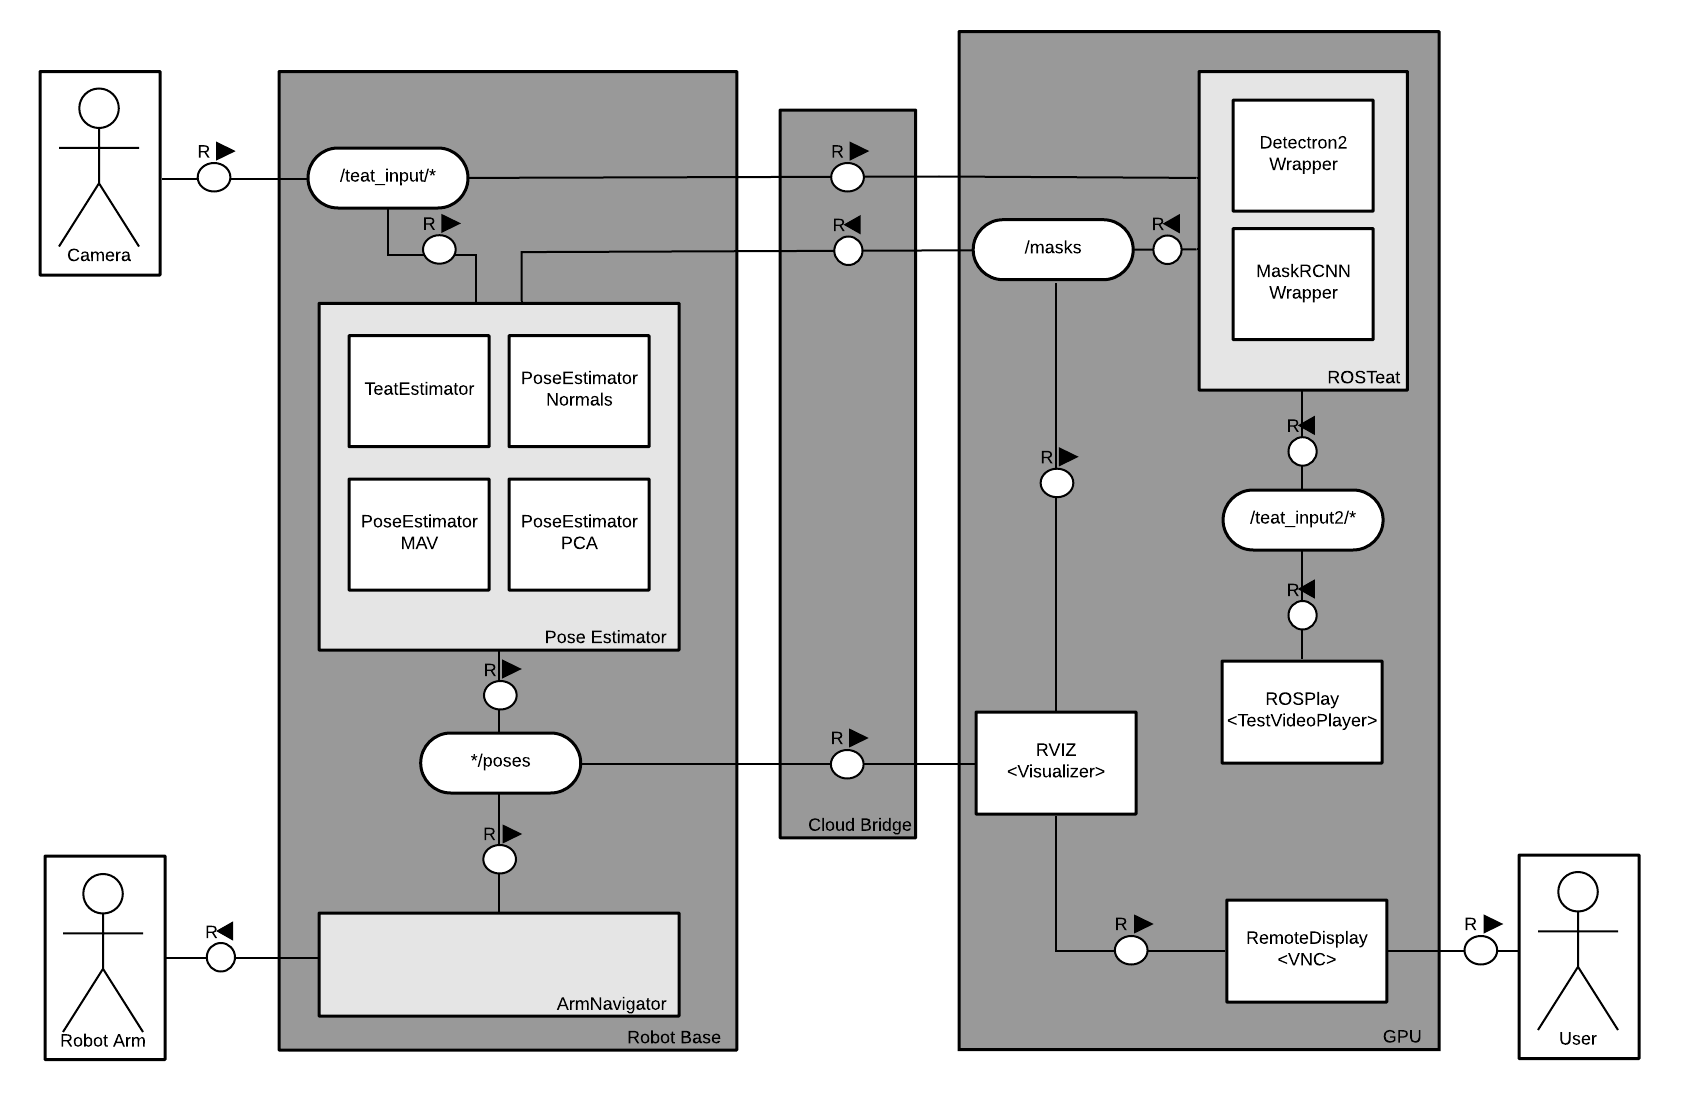
\includegraphics[width=.9\textwidth]{images/cow_fmc.png}
%         \caption{FMC diagram of the Pipeline's Architecture}
%         \label{fig:cow_fmc}
%     \end{figure}
% % \section{Software Design} 
% % \section{FMC Diagram}
% As a tool for designing a modular architecture, a domain model is used to help solve and understand the complexity in the system. The Fundamental Modeling Concepts (FMC) provide a framework for the comprehensive description of software-intensive systems \cite{FMCdiag}. 
% % Its block diagrams show the compositional structures as a composition of collaborating system components.
% In this framework, active system components are called agents and passive system components are called locations (storage, channels, queues; where information can be observed). The FMC diagram in Figure \ref{fig:cow_fmc} describes the high-level overview of the system's architecture, which illustrates the following agents and locations:
% \begin{itemize}
%     \item \textbf{Camera:} captures frames and publishes these as input for all the other components.
%     \item \textbf{User:} uses Rviz to visualize: the point cloud, the RGB image, the depth image, the segmented image of the cow teats and the 3D poses published.
%     \item \textbf{Robot Arm:} moves according to the instructions given by ArmNavigator. 
%     \item \textbf{PoseEstimator:} pose estimation algorithm that processes the information received from the camera and ROSTeat to predict 3D poses.
%     \item \textbf{ROSTeat Node:} processes images from the Camera node and segments the cow teats in the image.
%     \item \textbf{ArmNavigator:} manipulates the RobotArm according to the 3D poses published.
%     \item \textbf{ROSPlay <TestVideoPlayer> Node:} Behaves as a simulation/testing mechanism for reproducing the camera videos.
%     \item \textbf{RVIZ <Visualizer>:} ROS framework that allows the visualization of different ROS topics (RGB image, point cloud, etc.)
%     \item \textbf{RemoteDisplay <VNC>:} this is a browser-based graphical-d
%     esktop system that allows the visualization of RVIZ.
%     \item \textbf{/teat input/*:} channel where the camera input is published for other components to consume.
%     \item \textbf{/teat input2/*:} channel where the simulation video is published as input for other components to consume.
%     \item \textbf{/masks:} channel where the segmented cow teats are published.
%     \item \textbf{*/poses:} channel wehre the 3D cow teat poses are published.
% \end{itemize}
% One of the problems that appeared during this phase, was communicating the ROS (Robot Operating System) published messages across two networks. 
% % The ROS topics are the buses over which ROS nodes exchange messages (input images, masks, poses, etc.)\cite{2020ROStopics}.
% After thorough research it was found that ROS needs a routing mechanism that forwards the published topics (communication buses) from the Robot Base to the GPU and vice versa. The Cloud Bridge uses agents which are deployed on each network, to allow the intercommunication of topic messages. This allowed the deployment of the segmentation network in the GPU cluster, and the pose-estimation-related components in the Robot Base. 
% % The behavior and interactions of the main components (ROSTeat and Pose Estimator) are described in the following sections with more detail.

% % \section{Performance}\label{chap:3:performance}

% As part of the analysis process, one of the well established fundamental techniques is used: use cases. The use cases identified, which capture the black box requirements requirements for the given task, are 1) cow teat segmentation and 2) pose estimation. The sequence of activities and events described Table \ref{tab:use-segment} and Table \ref{tab:use-pose} takes special conditions and exceptions into consideration.

% \begin{longtable}{@{} p{3.5cm} p{10.5cm} @{}} \toprule
% \textbf{Use Case}       & \textbf{Segment Cow Teats from Image} \\ \midrule
% Actor                   & ROSTeat Node \\ \cmidrule{1-2}
% Description             & A cow teat is recognized from an image. \\ \cmidrule{1-2}
% Goal                    & Publish the cow teat masks present in received image. \\ \cmidrule{1-2}
% Preconditions           & An image exists. \\ 
%                         & ROSTeat node is running. \\ \cmidrule{1-2} 
% Postconditions          & A number of masks have been identified from image [0+]\\ \cmidrule{1-2} 
%                         & 1. The camera publishes an image. \\ 
% Basic Flow              & 2. The ROSTeat node consumes the image and predicts the cow teats in it. \\
%                         & 3. The ROSTeat node publishes the masks for future processing. \\ \cmidrule{1-2}
% Exceptions             & Image is not RGB \\ \bottomrule
% \caption{Use Case - Predict Masks} \label{tab:use-segment} \\
% \end{longtable}

% % \newpage
% \begin{longtable}{@{} p{3.5cm} p{10.5cm} @{}} \toprule
% \textbf{Use Case}       & \textbf{Estimate 3D Pose of Cow Teat} \\ \midrule
% Actor                   & Pose Estimator \\ \cmidrule{1-2}
% Description             & A cow teat pose is recognized from a tuple (image, point cloud, depth image, mask). \\ \cmidrule{1-2}
% Goal                    & Publish the cow teat poses for each message received. \\ \cmidrule{1-2}
% Preconditions           & An image exists. \\ 
%                         & ROSTeat node is running. \\ \cmidrule{1-2} 
% Postconditions          & A number of cow teat poses have been identified from image [0+]\\ \cmidrule{1-2} 
%                         & 1. The camera publishes an image AND ROSTeat node publishes the masks for the image (synchronized receival, stored as a tuple). \\ 
% Basic Flow              & 2. The Pose Estimator node consumes the tuple and predicts the cow teat poses in it. \\
%                         & 3. The Pose Estimator node publishes the poses for posterior attachment. \\ \cmidrule{1-2}
%                         \\
%                         \cmidrule{1-2}
% Exceptions             & TransformListener is empty \\ 
%                       & Any element in the tuple is empty and masks are not (data corruption). \\ \bottomrule
% \caption{Use Case - Predict Poses} \label{tab:use-pose} \\
% \end{longtable}


% % \subsection{Design}
% Given the nature of the recognition problem, it was determined that it is important to minimize assumptions on poses or camera angles (frame information) and account for the natural variation of the cow teats (udder morphology, colors, light conditions, etc.) as described in Section \ref{chap:2:melkroboter}.
% Figure \ref{fig:cow_topics} aids to illustrate a high-level overview of the communication fashion between components.
% Finally, given the modular design and message-based principles laid out, allowing any pose estimation algorithm to be used, the pipeline's proposed design is described below:

% \begin{enumerate}
%     \item The camera publishes information (RGB image, point cloud, depth image) into the input ROS topic channel, which is consumed to identify the position and size of salient objects.
%     \item The ROSTeat node subscribes to this input channel, uses the neural network to predict the cow teat masks and publishes them into a masks channel.
%     \item The Pose Estimator (plug-and-play component) consumes the masks that were published, and synchronizes it with the camera information (so it is all processed as a single message). The following pose estimation is algorithm-specific. Each pose estimation algorithm is described in detail in the following section. The poses are then published into a poses channel.
%     \item The robot consumes messages from the poses channel and moves 10-15 cm forward towards the indicated 3D poses, until it is 20-30 cm close to the pose estimations. Then the attachment process is initiated.
% \end{enumerate}

% \begin{figure}[!ht]
%     \centering
%     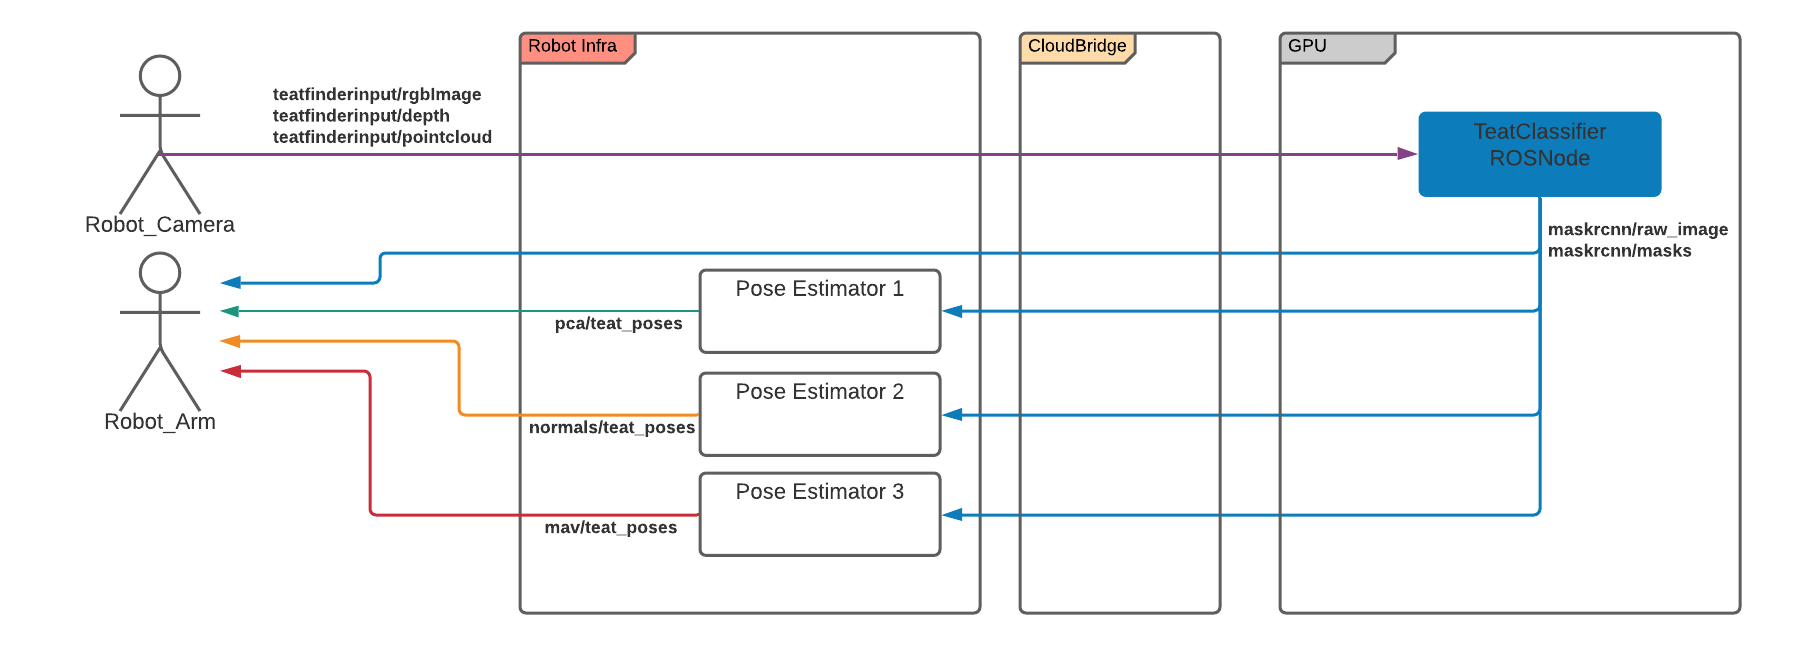
\includegraphics[width=1\textwidth]{images/cow_topics.png}
%     \caption{High-level flow diagram of the teat estimation pipeline.}
%     \label{fig:cow_topics}
% \end{figure}

% %  As explained in Section \ref{chap:3:architecture} the messages must go through a Cloud Bridge to be able to connect the robot's ROS local topics with the GPU ROS topics. 


% As described above, the interactions between the camera and the recognition components depend on the messages received (images, masks). In order to improve the efficiency of the development process, the ROSPlay component was introduced to allow the repetition of camera frames from a ROSbag (ROS format for a video file). A ROSBag is then used for data generation, algorithm training and testing. One of the problems encountered in this phase was that the generated ROSbags are up to 20 GB in size. These ROSBags are generated in the ROS Base and have to be transferred over the network to the development environment (local laptop or GPU cluster). This can be time consuming but it is required for the development.  
% Appendix \ref{appendix:cow_design} additionally provides an alternative illustration for the processing pipeline.

